\section{METODOLOGIA}
A execução do projeto fundamenta-se no Ciclo Básico de Produção de Jogos proposto por Heather Chandler \cite{Chandler2009}, Fig. \ref{fig:ciclochandler}, adotando uma abordagem cíclica e iterativa. A escolha dessa metodologia justifica-se pela necessidade de equilibrar a fidelidade científica com a jogabilidade de um jogo sério eficaz.

\begin{figure}[h]
    \centering
    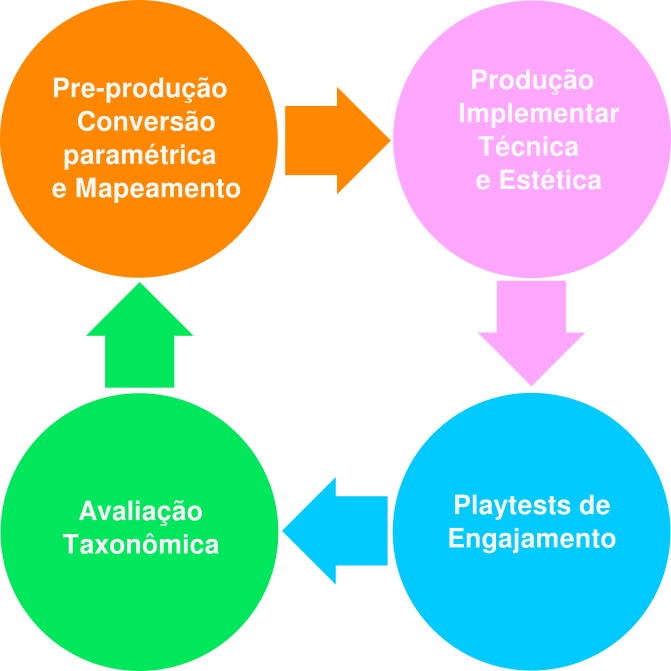
\includegraphics[width=0.4\textwidth]{images/ciclochandler.png}
    \caption{Ciclo Básico de Produção de Jogos. Fonte: adaptado de \cite{Chandler2009}.}
    \label{fig:ciclochandler}
\end{figure}


\subsection{Pré-produção e transposição didática}
A seleção dos conteúdos para o \textit{Alchemon} foi estruturada para refletir as competências de análise de fenômenos naturais da BNCC (competência EM13CNT201 da BNCC) \cite{BNCC26}, utilizando a clareza prática e experimental do currículo internacional IGCSE \cite{igcse_chemistry_2023}. 

No sistema de jogo, essa progressão curricular dita a curva de dificuldade e o desbloqueio de mecânicas:
\begin{itemize}
    \item Atomística e Tabela Periódica: Estruturam as propriedades fundamentais das criaturas (\textit{status} base de HP, ataque e defesa determinados por raio atômico e eletronegatividade).
    \item Ligações Químicas: Atuam como sistemas de sinergia em batalhas de equipe e mecânicas de evolução por fusão (combinação de elementos para formar substâncias iônicas ou covalentes).
\end{itemize}

O diferencial desta etapa reside na transformação das propriedades periódicas em regras de mecânica e atributos sistêmicos, de modo que o domínio das leis da Química se torne condição essencial para o sucesso estratégico no jogo. As mecânicas e a fundamentação teórica serão expandidas no \textit{High-Concept Document} (HCD) anexado.

\subsection{Produção e identidade visual}
A produção ocorrerá de forma iterativa, dividindo-se entre a lógica sistêmica e a construção estética. A implementação técnica das mecânicas principais e do sistema de progressão pedagógica será realizada no motor de jogos Godot \cite{Godot2024}, escolhido por sua versatilidade e sua natureza (\textit{open-source}). Em um segundo ciclo iterativo, o foco voltar-se-á para a identidade visual das criaturas, visando criar representações únicas e memoráveis para os elementos químicos.

Utilizar-se-á o \textit{software} Blender \cite{Blender2024} para modelagem 3D e o Krita \cite{Krita2024} para texturização e arte 2D. A estética será deliberadamente inspirada no estilo gráfico de \textit{Digimon World}, adotando arquétipos que facilitem a memorização visual e a conexão psicológica do jogador com sua coleção \cite{Gomez2019}. Essa abordagem visar-se-á a reduzir a carga cognitiva estranha e aumentar a curiosidade, estimulando a aprendizagem tangencial espontânea \cite{Portnow2012}.

\subsection{Testes e engajamento volitivo}
Os ciclos de testes concentrar-se-ão em usabilidade e diversão, validando se o Alchemon atenderá ao critério de ser engajador sem que a intencionalidade pedagógica prejudique o engajamento volitivo do jogador \cite{Jacobs2021}. Buscar-se-á confirmar se o jogo promove a satisfação das necessidades psicológicas básicas, especificamente autonomia e competência \cite{Ryan1985}, permitindo que o estudante sinta-se o agente de seu próprio progresso.

\section{IDENTIFICAÇÃO E RESOLUÇÃO DO PROBLEMA}

O ensino de Química, especialmente no que se refere ao domínio da Tabela Periódica, enfrenta uma persistente dificuldade de aprendizagem associada à predominância de práticas pedagógicas tradicionais baseadas na memorização mecânica, em detrimento de abordagens que promovam o engajamento ativo dos estudantes \cite{Latonio2023}. Nesse contexto, a periodicidade química é frequentemente percebida como um conteúdo abstrato e de alta complexidade, sendo abordada por meio de estratégias de memorização que não favorecem a construção de uma compreensão significativa de suas relações estruturais e funcionais \cite{Lima2010}.

Evidências empíricas demonstram a gravidade dessa lacuna, pois estudos diagnósticos revelam que estudantes de nível médio frequentemente falham em atingir o limiar básico de proficiência de 75\% em testes de compreensão da Tabela Periódica \cite{Latonio2023}. No cenário brasileiro, essa dificuldade é corroborada pelos resultados do PISA 2022, que indicam que apenas 45\% dos estudantes atingem o nível mínimo de proficiência em ciências \cite{OECD2023}.

Além das dificuldades cognitivas, a predominância de métodos expositivos e centrados no professor impacta negativamente a motivação dos estudantes e a retenção de conhecimento a longo prazo. A literatura aponta que a aprendizagem significativa está diretamente relacionada à satisfação de necessidades psicológicas básicas, como autonomia, competência e pertencimento \cite{Ryan1985}. No entanto, o modelo tradicional de ensino tende a limitar a participação ativa do estudante, o que reduz sua agência no processo de aprendizagem e contribui para o desinteresse generalizado pelos conteúdos científicos \cite{SilvaFilho2023}.

Nesse panorama, o desenvolvimento do projeto Alchemon justifica-se como uma tentativa de mitigar essas barreiras por meio de um jogo sério \cite{Plass2020}. A proposta busca converter a passividade da recepção de conteúdo em uma experiência de descoberta ativa, utilizando a estética de captura de criaturas para transformar o estudo da Química em uma ferramenta estratégica de progressão e maestria.

\subsection{Proposta de solução}
O projeto Alchemon propõe a convergência sinérgica entre a Teoria da Autodeterminação (SDT) \cite{Ryan1985}, a Aprendizagem Significativa (TAS) \cite{Ausubel1963} e a Aprendizagem Tangencial \cite{Portnow2012} para mitigar as barreiras do ensino tradicional, Fig. \ref{fig:cicloteorico}. Para evitar o fenômeno do \enquote{brócolis coberto de chocolate} \cite{Plass2020, Lorenzatti2020}, o jogo diferencia-se de abordagens educativas convencionais ao buscar uma sólida integração intrínseca (\textit{intrinsic integration}) \cite{Vahlo2023}. Assegura-se, assim, que as mecânicas lúdicas e o conteúdo científico sejam indissociáveis \cite{Plass2020}, de modo que as leis da Química não funcionem como obstáculos ou interrupções didáticas, mas constituam a própria lógica de interação e as condições de vitória do sistema \cite{Mozelius2017}.

Sob essa lógica, a solução concentra-se em satisfazer as necessidades psicológicas de autonomia e competência por meio de \textit{feedbacks} de maestria \cite{Shi2016}, transformando o conteúdo acadêmico em uma ferramenta de empoderamento estratégico \cite{Plass2020, Shi2016}. Isso garante que o jogador busque voluntariamente informações técnicas para obter vantagens \textit{in-game} \cite{Vahlo2023}, convertendo o interesse espontâneo em desempenho acadêmico mensurável \cite{LimadaCostaJunior2022}.

Para materializar esse engajamento, o projeto apoia-se na curiosidade inerente ao gênero \textit{Creature Capture} \cite{Portnow2012}, preenchendo uma lacuna teórica e estética identificada a partir dos trabalhos correlatos. Enquanto o \textit{ChemCraft} concentra-se em reações diretas e o \textit{ChemCaper} em um RPG tradicional, o Alchemon inova ao adotar uma estética de criaturas única para cada elemento químico. Superando os modelos baseados apenas em cartas ou fórmulas geométricas, essa escolha de design atua como um organizador prévio \cite{Ausubel1963}: as mecânicas de captura facilitam a memorização visual e ancoram os novos conhecimentos químicos de forma não arbitrária e substantiva, conforme os preceitos da Teoria da Aprendizagem Significativa (TAS) \cite{Ausubel1963, Espirito2020}.

Além disso, o Alchemon propõe um sistema de habilidades químicas dinâmicas baseado em propriedades periódicas, superando os modelos lineares vistos em outros trabalhos. Assim, o projeto justifica-se ao oferecer um método de estudo adaptado aos nativos digitais brasileiros, integrando as necessidades de autonomia e competência da Teoria da Autodeterminação (SDT) \cite{Ryan1985} ao ensino da Tabela Periódica no Ensino Médio.

Uma proposta incial do \textit{Game Design Document} (GDD) esta anexada\footnote{Link para o GDD http://bit.ly/43sUnRf}

\begin{figure}
    \centering
    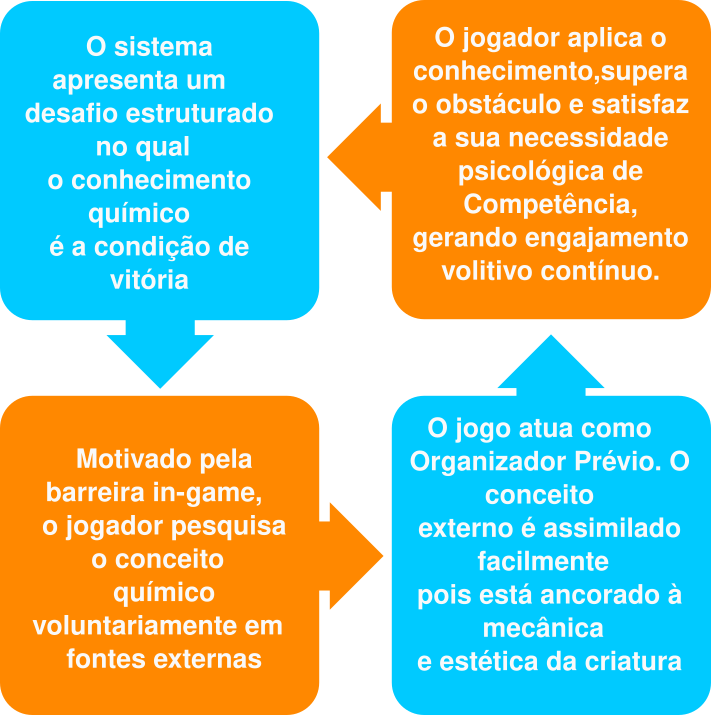
\includegraphics[width=0.4\textwidth]{images/cicloteorico.png}
    \caption{Ciclo educacional do projeto. Fonte: elaborado pelo autor.}
    \label{fig:cicloteorico}
\end{figure}
